% ============================================================
% 34-bezier-curvature-explained.tex
% Compile with:  pdflatex -shell-escape 34-bezier-curvature-explained.tex
% Both PNGs must be in the same folder. Run twice for TOC.
% ============================================================

\documentclass[12pt, a4paper]{article}

\usepackage[T1]{fontenc}
\usepackage[utf8]{inputenc}
\usepackage{lmodern}
\usepackage[top=2.5cm, bottom=2.5cm, left=2.8cm, right=2.8cm]{geometry}
\usepackage{graphicx}
\usepackage{float}
\usepackage[dvipsnames]{xcolor}

\definecolor{codebg}{RGB}{248,248,248}
\definecolor{rulecolor}{RGB}{180,180,180}
\definecolor{examplebg}{RGB}{240,248,255}
\definecolor{examplerule}{RGB}{100,149,237}
\definecolor{notebg}{RGB}{255,250,230}
\definecolor{noterule}{RGB}{210,180,50}
\definecolor{samebg}{RGB}{245,245,245}
\definecolor{samerule}{RGB}{160,160,160}

\usepackage{minted}
\setminted[julia]{
  bgcolor=codebg, frame=leftline, framerule=1.5pt,
  rulecolor=rulecolor, linenos=false, fontsize=\small,
  breaklines=true, tabsize=4, style=friendly,
}

\usepackage{amsmath}
\usepackage{amssymb}
\usepackage{tikz}
\usetikzlibrary{shapes.geometric, arrows.meta, positioning}
\usepackage{mdframed}

\newmdenv[backgroundcolor=examplebg, linecolor=examplerule,
  linewidth=1.5pt, leftline=true, rightline=false,
  topline=false, bottomline=false,
  innerleftmargin=10pt, innerrightmargin=8pt,
  innertopmargin=6pt, innerbottommargin=6pt,
  skipabove=6pt, skipbelow=4pt]{examplebox}

\newmdenv[backgroundcolor=notebg, linecolor=noterule,
  linewidth=1.5pt, leftline=true, rightline=false,
  topline=false, bottomline=false,
  innerleftmargin=10pt, innerrightmargin=8pt,
  innertopmargin=6pt, innerbottommargin=6pt,
  skipabove=6pt, skipbelow=4pt]{notebox}

\newmdenv[backgroundcolor=samebg, linecolor=samerule,
  linewidth=1.5pt, leftline=true, rightline=false,
  topline=false, bottomline=false,
  innerleftmargin=10pt, innerrightmargin=8pt,
  innertopmargin=6pt, innerbottommargin=6pt,
  skipabove=6pt, skipbelow=4pt]{samebox}

\usepackage[colorlinks=true, linkcolor=black, urlcolor=MidnightBlue]{hyperref}
\usepackage{booktabs}
\usepackage{needspace}
\usepackage{parskip}
\usepackage{titlesec}
\usepackage{fancyhdr}
\usepackage{datetime2}

\titleformat{\section}
  {\large\bfseries\color{MidnightBlue}}{\thesection.}{0.6em}{}
  [\vspace{-4pt}\rule{\linewidth}{0.4pt}]
\titleformat{\subsection}
  {\normalsize\bfseries\color{BrickRed}}{\thesubsection.}{0.5em}{}
\titleformat{\subsubsection}
  {\normalsize\bfseries}{\thesubsubsection.}{0.5em}{}

\pagestyle{fancy}
\fancyhf{}
\rhead{\textcolor{gray}{\small 34-bezier-curvature-explained}}
\lhead{\textcolor{gray}{\small B\'ezier Curvature --- GLMakie}}
\cfoot{\thepage}
\renewcommand{\headrulewidth}{0.3pt}

\newcommand{\cd}[1]{\texttt{#1}}

\title{%
  \vspace{1cm}
  {\LARGE\bfseries B\'ezier Curve + Curvature Comb}\\[0.4em]
  {\large Generic 2-D / 3-D --- GLMakie}\\[0.4em]
  {\large Code and Plot Explanation for Julia Beginners}\\[0.4em]
  {\normalsize\texttt{34-bezier-curvature.jl}}
}
\author{E.R.\ Nurwijayadi}
\date{\DTMtoday}

\begin{document}

\maketitle
\thispagestyle{empty}

\begin{center}
\textit{Directed and curated by E.R.\ Nurwijayadi.
Code and explanations AI-generated.}
\end{center}

\begin{center}
\begin{minipage}{0.85\textwidth}
\small
This document explains \cd{34-bezier-curvature.jl}.
It extends \cd{31-bezier-generic.jl} with one major addition:
the \textbf{curvature comb} --- a visual representation
of how much the curve bends at each point.
New concepts: derivative control points, the curvature
formula, the curvature normal vector in 2-D and 3-D,
automatic comb scaling via quantile, and the
\cd{draw\_comb!} function.
The \cd{draw\_and\_show} body and all drawing layers are
otherwise identical to script~31.
\end{minipage}
\end{center}

\vspace{1em}\hrule\vspace{1.5em}
\tableofcontents
\newpage


% =============================================================
\needspace{8\baselineskip}
\section{The Two Plots}
% =============================================================

\needspace{5\baselineskip}
\subsection{Case 1 --- Quadratic 2-D with Curvature Comb}

\begin{figure}[H]
  \centering
  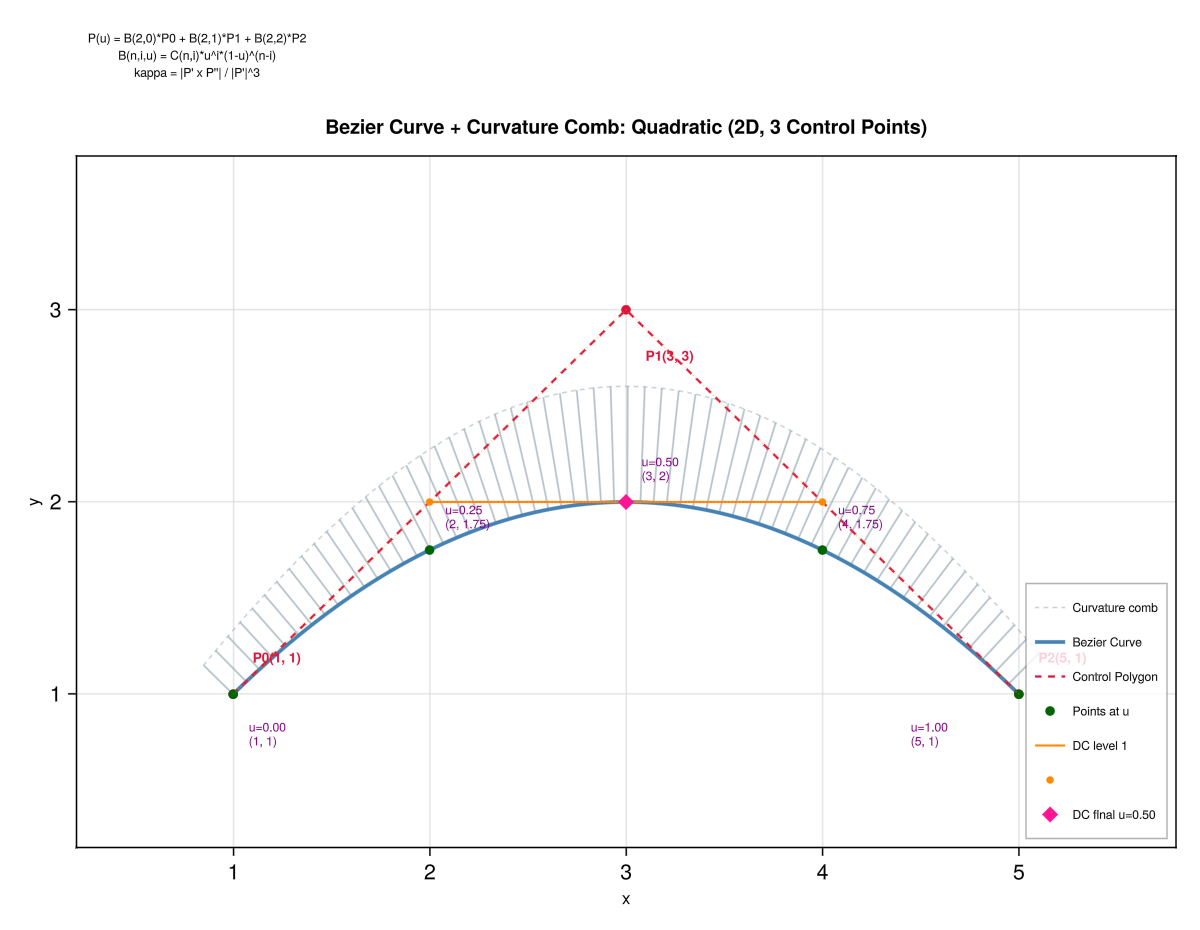
\includegraphics[width=0.92\linewidth]{34-bezier-curvature-quadratic-2d.png}
  \caption{Case~1: quadratic B\'ezier with curvature comb in 2-D.
           The grey fan of spikes above the curve shows that
           curvature is highest near the centre and falls
           off symmetrically toward the endpoints.}
\end{figure}

\needspace{5\baselineskip}
\subsection{Case 2 --- Quartic 3-D with Curvature Comb}

\begin{figure}[H]
  \centering
  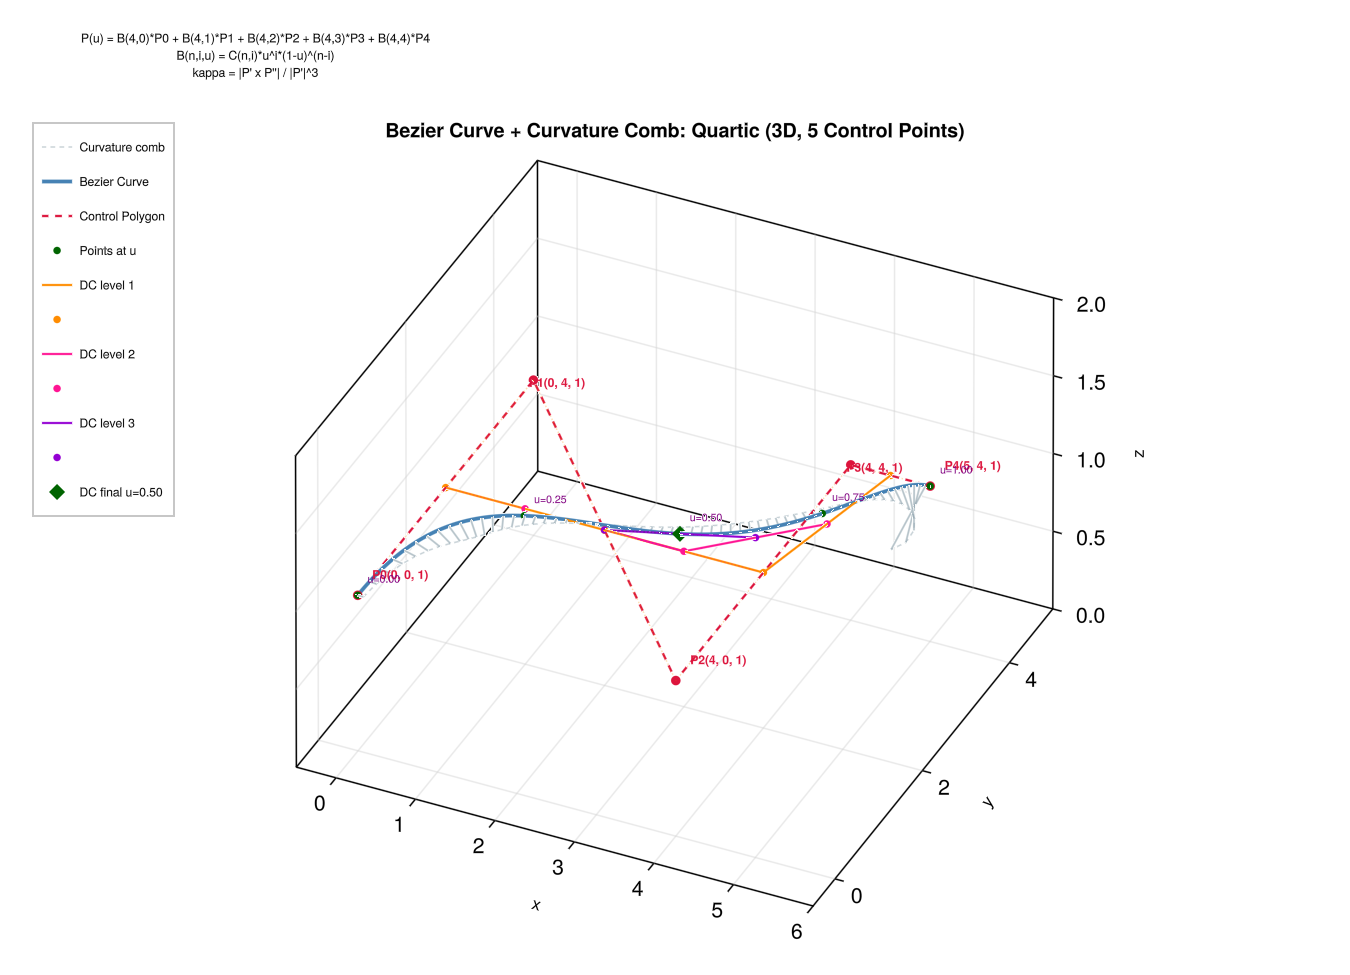
\includegraphics[width=0.92\linewidth]{34-bezier-curvature-quartic-3d.png}
  \caption{Case~2: quartic B\'ezier with curvature comb in 3-D.
           The grey spikes point along the principal normal
           of the curve at each sample point.}
\end{figure}


% =============================================================
\needspace{8\baselineskip}
\section{What Is Curvature?}
% =============================================================

\textit{Before reading the code, understand what is being measured.}

The \textbf{curvature} $\kappa$ of a curve at a point
measures how sharply the curve bends there.
A straight line has $\kappa = 0$.
A circle of radius $r$ has constant $\kappa = 1/r$.
A tighter bend (smaller radius of curvature) gives a
larger $\kappa$.

For a parametric curve $P(u)$ with first derivative
$P'(u)$ and second derivative $P''(u)$, curvature is:
\[
  \kappa = \frac{|P' \times P''|}{|P'|^3}
\]

In 2-D the cross product produces a scalar
(the $z$-component of the 3-D cross product),
so $|P' \times P''| = |P'_x P''_y - P'_y P''_x|$.
In 3-D it produces a vector, and we take its norm.

The \textbf{curvature comb} is a standard visualisation
technique in computer-aided design.
At each point on the curve, a spike is drawn perpendicular
to the tangent, with length proportional to $\kappa$.
The envelope connecting the spike tips reveals how
smoothly curvature changes along the curve.

\begin{notebox}
\textbf{Reading the 2-D plot:}
The spikes above the curve are tallest near $u = 0.5$
(the peak of the arc, where bending is greatest) and
shrink symmetrically toward the endpoints.
The quadratic B\'ezier has \emph{constant} curvature for this
symmetric configuration, so the comb tips trace a nearly
uniform arc --- the envelope is smooth and even.
\end{notebox}


% =============================================================
\needspace{8\baselineskip}
\section{New Imports}
% =============================================================

\begin{minted}{julia}
using LinearAlgebra
using Statistics
\end{minted}

Two new standard library packages:

\textbf{\cd{LinearAlgebra}:} provides \cd{norm} (vector
magnitude) and \cd{cross} (3-D cross product).
Both are used in curvature computation.

\textbf{\cd{Statistics}:} provides \cd{quantile},
used to auto-scale the comb height.
These are part of Julia's standard library ---
no \cd{Pkg.add} needed.


% =============================================================
\needspace{8\baselineskip}
\section{The Extended \texttt{BezierCurve} Struct}
% =============================================================

\begin{minted}{julia}
struct BezierCurve
    points  ::Matrix{Float64}
    n       ::Int
    degree  ::Int
    dim     ::Int
    d1_pts  ::Matrix{Float64}          # (n-1 x dim)
    d2_pts  ::Union{Matrix{Float64}, Nothing}  # (n-2 x dim)
end

function BezierCurve(points::Matrix{Float64})
    n      = size(points, 1)
    deg    = n - 1
    dim    = size(points, 2)
    d1_pts = deg .* diff(points, dims=1)
    d2_pts = size(d1_pts, 1) > 1 ?
             (deg - 1) .* diff(d1_pts, dims=1) : nothing
    BezierCurve(points, n, deg, dim, d1_pts, d2_pts)
end
\end{minted}

\needspace{5\baselineskip}
\subsection{Two new fields: \texttt{d1\_pts} and \texttt{d2\_pts}}

These store the \textbf{derivative control points} ---
the control points of the first and second derivative
curves.

For a B\'ezier curve of degree $n$ with control points
$P_0, \ldots, P_n$, the first derivative is itself a
B\'ezier curve of degree $n-1$ with control points:
\[
  Q_i = n \cdot (P_{i+1} - P_i), \quad i = 0, \ldots, n-1
\]
The second derivative is a B\'ezier of degree $n-2$
with control points derived similarly from $Q_i$.

This means the derivative at any $u$ can be evaluated
using the same Bernstein machinery --- just with different
control points and degree.

\textbf{\cd{d2\_pts ::Union\{Matrix\{Float64\}, Nothing\}}:}
For a linear curve (degree 1, two control points),
\cd{d1\_pts} has one row --- a single point, not a
curve --- and there is no second derivative in the
same sense.
\cd{Union\{Matrix\{Float64\}, Nothing\}} means the field
can hold either a matrix \emph{or} the special value
\cd{nothing}.
This is Julia's way of expressing an optional value.

\needspace{5\baselineskip}
\subsection{\texttt{diff(points, dims=1)} --- the derivative shortcut}

\begin{minted}{julia}
d1_pts = deg .* diff(points, dims=1)
\end{minted}

\cd{diff(A, dims=1)} computes differences between
consecutive rows of matrix \cd{A}.
For a $5\times3$ matrix it returns a $4\times3$ matrix
where row $i$ is \cd{A[i+1,:] - A[i,:]}.

Multiplied by \cd{deg} (broadcast \cd{.*}), this gives
exactly the first derivative control points $Q_i = n(P_{i+1}-P_i)$.

\begin{examplebox}
\textbf{For Case~1 (quadratic 2-D):}

\cd{points} $= \begin{bmatrix}1&1\\3&3\\5&1\end{bmatrix}$, \quad \cd{deg = 2}

\cd{diff(points, dims=1)} $= \begin{bmatrix}2&2\\2&-2\end{bmatrix}$

\cd{d1\_pts = 2 .* ...} $= \begin{bmatrix}4&4\\4&-4\end{bmatrix}$

So $Q_0 = [4, 4]$ and $Q_1 = [4, -4]$.

\medskip
\cd{diff(d1\_pts, dims=1)} $= \begin{bmatrix}0&-8\end{bmatrix}$

\cd{d2\_pts = 1 .* ...} $= \begin{bmatrix}0&-8\end{bmatrix}$
\quad (one row --- degree 0 constant)

This means $P''(u) = [0, -8]$ for all $u$ ---
constant second derivative, confirming that a quadratic
B\'ezier has constant curvature under symmetric conditions.
\end{examplebox}


% =============================================================
\needspace{8\baselineskip}
\section{The Math Functions}
% =============================================================

\needspace{5\baselineskip}
\subsection{\texttt{eval\_poly} --- shared evaluator}

\begin{minted}{julia}
function eval_poly(pts::Matrix{Float64}, u::Float64)
    n = size(pts, 1) - 1
    sum(bernstein(n, i-1, u) .* pts[i,:] for i in 1:size(pts,1))
end
\end{minted}

A generalised version of \cd{bz\_point} from script~31.
It evaluates a B\'ezier curve defined by \emph{any}
control point matrix at parameter \cd{u}, computing
the degree from the number of rows.
This makes it reusable for the original curve
(\cd{bz.points}), the first derivative (\cd{bz.d1\_pts}),
and the second derivative (\cd{bz.d2\_pts}).

\needspace{5\baselineskip}
\subsection{\texttt{bz\_d1} and \texttt{bz\_d2}}

\begin{minted}{julia}
function bz_d1(bz::BezierCurve, u::Float64)
    eval_poly(bz.d1_pts, u)
end

function bz_d2(bz::BezierCurve, u::Float64)
    isnothing(bz.d2_pts) ? zeros(bz.dim) : eval_poly(bz.d2_pts, u)
end
\end{minted}

\cd{bz\_d1} evaluates the first derivative $P'(u)$ by
calling \cd{eval\_poly} on the derivative control points.

\cd{bz\_d2} handles the \cd{nothing} case:
if \cd{d2\_pts} is \cd{nothing} (for a linear curve),
it returns a zero vector, which makes curvature zero
everywhere --- correct, since a straight line has no bending.

\cd{isnothing(x)} returns \cd{true} if \cd{x} is \cd{nothing}.

\begin{examplebox}
\textbf{For Case~1 at $u = 0.5$:}

\cd{d1\_pts} $= \begin{bmatrix}4&4\\4&-4\end{bmatrix}$, degree 1.

\cd{eval\_poly(d1\_pts, 0.5)} evaluates a linear
B\'ezier with these two points:
$0.5 \times [4,4] + 0.5 \times [4,-4] = [4, 0]$

So $P'(0.5) = [4, 0]$ --- the tangent at the peak
is horizontal. \checkmark

\cd{d2\_pts} $= \begin{bmatrix}0&-8\end{bmatrix}$, degree 0.

\cd{eval\_poly(d2\_pts, 0.5)} $= [0, -8]$

So $P''(0.5) = [0, -8]$ for all $u$. \checkmark
\end{examplebox}

\needspace{5\baselineskip}
\subsection{\texttt{bz\_curvature} --- the curvature formula}

\begin{minted}{julia}
function bz_curvature(bz::BezierCurve, u::Float64)
    d1    = bz_d1(bz, u)
    d2    = bz_d2(bz, u)
    speed = norm(d1)
    speed < 1e-10 && return 0.0
    if bz.dim == 2
        abs(d1[1]*d2[2] - d1[2]*d2[1]) / speed^3
    else
        norm(cross(d1, d2)) / speed^3
    end
end
\end{minted}

\textbf{\cd{speed = norm(d1)}:}
The speed is the magnitude of the velocity vector $P'(u)$.
It appears as $|P'|$ in the denominator of the curvature formula.

\textbf{\cd{speed < 1e-10 \&\& return 0.0}:}
A short-circuit guard: if the curve has zero speed
(a cusp or stationary point), curvature is undefined.
Returning 0.0 prevents division by zero.
The \cd{\&\&} operator evaluates the right side only if the
left side is \cd{true} --- a concise way to write
\cd{if speed < 1e-10; return 0.0; end}.

\textbf{2-D branch:}
The curvature formula uses the 2-D scalar cross product
$|P'_x P''_y - P'_y P''_x|$, the $z$-component of the
3-D cross product when both vectors lie in the $xy$-plane.

\textbf{3-D branch:}
\cd{cross(d1, d2)} computes the 3-D cross product vector.
\cd{norm(...)} takes its magnitude.
This is the standard formula $\kappa = |P' \times P''| / |P'|^3$.

\begin{examplebox}
\textbf{Curvature at $u = 0.5$ for Case~1:}

$P'(0.5) = [4, 0]$, \quad $P''(0.5) = [0, -8]$

$\text{speed} = \sqrt{4^2 + 0^2} = 4$

$|P'_x P''_y - P'_y P''_x| = |4 \times (-8) - 0 \times 0| = 32$

$\kappa(0.5) = \dfrac{32}{4^3} = \dfrac{32}{64} = 0.5$

This means the radius of curvature at the peak is $1/0.5 = 2$
data units --- a fairly tight bend for a curve spanning
4 units horizontally.
\end{examplebox}


% =============================================================
\needspace{8\baselineskip}
\section{\texttt{draw\_comb!} --- Drawing the Curvature Comb}
% =============================================================

\begin{minted}{julia}
function draw_comb!(ax, bz::BezierCurve, u_vals, curve_pts,
                    kappas, comb_scale, is_3d)
    step  = max(1, length(u_vals) ÷ 60)
    u_sub = u_vals[1:step:end]
    m     = length(u_sub)

    base = hcat([bz_point(bz, u) for u in u_sub]...)'
    d1v  = hcat([bz_d1(bz, u)   for u in u_sub]...)'
    d2v  = hcat([bz_d2(bz, u)   for u in u_sub]...)'
    kap  = [bz_curvature(bz, u) for u in u_sub]
    tips = similar(base)
    ...
end
\end{minted}

\needspace{5\baselineskip}
\subsection{Naming convention: \texttt{!} means mutates the axis}

The function is named \cd{draw\_comb!} with an exclamation
mark.
In Julia, the \cd{!} suffix is a naming convention indicating
that the function \emph{mutates} one of its arguments ---
here, it adds plot elements to \cd{ax} in place.
This mirrors Makie's own \cd{lines!}, \cd{scatter!},
\cd{text!} convention.
The \cd{!} is not required by the language; it is a
community convention that signals mutation.

\needspace{5\baselineskip}
\subsection{Subsampling with integer division (\texttt{\textbackslash div})}

\begin{minted}{julia}
step  = max(1, length(u_vals) ÷ 60)
u_sub = u_vals[1:step:end]
\end{minted}

Drawing one spike per curve sample (300 spikes) would
produce a dense, unreadable comb.
\cd{length(u\_vals) \textbackslash div{} 60} performs \textbf{integer division}
(the \cd{\textbackslash div} operator, typed as \cd{\\} + \cd{div} + Tab in Julia) to
calculate a step size that gives roughly 60 evenly
spaced spikes.
\cd{max(1, ...)} ensures the step is at least 1.
\cd{u\_vals[1:step:end]} slices the array with a stride
of \cd{step}.

\needspace{5\baselineskip}
\subsection{\texttt{similar(base)} --- allocating an output matrix}

\begin{minted}{julia}
tips = similar(base)
\end{minted}

\cd{similar(A)} allocates a new matrix with the same
shape and element type as \cd{A}, but with
\emph{uninitialised} values.
It is equivalent to \cd{zeros(size(base,1), size(base,2))}
but slightly more efficient since it skips the
zero-fill step.
\cd{tips} will hold the endpoint of each curvature spike.

\needspace{5\baselineskip}
\subsection{\texttt{LinearAlgebra} and \texttt{Statistics} functions used}

\subsubsection{\texttt{norm(v)} --- vector magnitude}

\cd{norm(v)} computes the Euclidean length of a vector:
\[
  \|\mathbf{v}\| = \sqrt{v_1^2 + v_2^2 + \cdots + v_n^2}
\]

In the comb code it appears as \cd{norm(d1v[i,:])}
(the speed $\|P'(u)\|$) and \cd{norm(N\_raw)}
(the length of the raw principal normal vector).
It also appears in \cd{bz\_curvature} as
\cd{norm(d1)} for the speed denominator and
\cd{norm(cross(d1, d2))} for the cross product magnitude.

\subsubsection{\texttt{cross(a, b)} --- vector cross product}

\cd{cross(a, b)} computes the 3-D cross product of two
vectors using the $3\times3$ determinant:
\[
  \mathbf{a} \times \mathbf{b}
  = \begin{vmatrix}
      \mathbf{i} & \mathbf{j} & \mathbf{k} \\
      a_1 & a_2 & a_3 \\
      b_1 & b_2 & b_3
    \end{vmatrix}
  = \begin{bmatrix}
      a_2 b_3 - a_3 b_2 \\
      a_3 b_1 - a_1 b_3 \\
      a_1 b_2 - a_2 b_1
    \end{bmatrix}
\]

The result is a vector \emph{perpendicular} to both
$\mathbf{a}$ and $\mathbf{b}$, with magnitude:
\[
  \|\mathbf{a} \times \mathbf{b}\| = \|\mathbf{a}\|\,\|\mathbf{b}\|\sin\theta
\]
where $\theta$ is the angle between them.
This magnitude is used directly in the curvature formula:
\begin{minted}{julia}
kappa = norm(cross(d1, d2)) / speed^3
\end{minted}
which corresponds to:
\[
  \kappa = \frac{\|P'(u) \times P''(u)\|}{\|P'(u)\|^3}
\]

\subsubsection{\texttt{quantile(data, p)} --- statistical threshold}

\cd{quantile(data, p)} returns the value below which
a fraction $p$ of the data falls.
\cd{p = 0.95} gives the 95th percentile: the value
that is larger than 95\% of all observations.

\begin{minted}{julia}
kap_95 = quantile(kappas, 0.95)
\end{minted}

Here it provides a robust upper reference for curvature ---
ignoring the top 5\% of outlier values that can appear
at curve endpoints where the formula is sensitive to
small numerical errors.
The comb is then scaled so that a spike at \cd{kap\_95}
reaches 15\% of the curve extent.

\needspace{5\baselineskip}
\subsection{The 2-D normal vector --- four steps}

\begin{minted}{julia}
for i in 1:m
    spd = norm(d1v[i,:])
    spd = spd > 1e-10 ? spd : 1e-10
    T   = d1v[i,:] / spd        # unit tangent
    N   = [-T[2], T[1]]         # unit normal (90-degree rotation)
    tips[i,:] = base[i,:] .+ comb_scale * kap[i] .* N
end
\end{minted}

Each iteration computes the spike tip in four steps.

\textbf{Step 1 --- Speed} $\|\mathbf{v}\| = \|P'(u)\|$
\[
  \text{\cd{spd}} = \|\mathbf{d1}\|
  = \sqrt{d1_x^2 + d1_y^2}
\]
\cd{norm(d1v[i,:])} returns the Euclidean length of the
velocity vector at this sample point.
The guard \cd{spd > 1e-10 ? spd : 1e-10} prevents
division by zero at a cusp.

\textbf{Step 2 --- Unit Tangent} $T$
\[
  T = \frac{P'(u)}{\|P'(u)\|}
  \qquad
  \text{\cd{T = d1v[i,:] / spd}}
\]
Dividing the velocity vector by its own length produces
a vector of length exactly 1 pointing in the direction
of travel.

\textbf{Step 3 --- Unit Normal} $N$
\[
  N = \begin{bmatrix}-T_y \\ T_x\end{bmatrix}
  \qquad
  \text{\cd{N = [-T[2], T[1]]}}
\]
Rotating a 2-D unit vector $[T_x, T_y]$ by
$90^{\circ}$ counter-clockwise gives $[-T_y, T_x]$.
This is the unit normal vector perpendicular to the
tangent, pointing toward the centre of curvature.

\textbf{Step 4 --- Tip position}
\[
  \text{tip} = P(u) + s \cdot \kappa \cdot N
  \qquad
  \text{\cd{tips[i,:] = base[i,:] .+ comb\_scale * kap[i] .* N}}
\]
The spike endpoint is displaced from the curve point
by \cd{comb\_scale} $\times$ $\kappa$ in the normal direction.
A higher curvature produces a longer spike.

\needspace{5\baselineskip}
\subsection{The 3-D principal normal vector}

\begin{minted}{julia}
for i in 1:m
    d1i   = d1v[i,:]
    d2i   = d2v[i,:]
    N_raw = cross(cross(d1i, d2i), d1i)
    n_mag = norm(N_raw)
    N     = n_mag > 1e-10 ? N_raw / n_mag : zeros(3)
    tips[i,:] = base[i,:] .+ comb_scale * kap[i] .* N
end
\end{minted}

In 3-D, the normal direction is the \textbf{principal normal}:
the direction in which the curve is turning.
The formula $N_\text{raw} = (P' \times P'') \times P'$ gives the
component of $P''$ perpendicular to $P'$, which points
toward the centre of curvature.
After normalising, this is the unit principal normal.

The inner cross product $P' \times P''$ uses the
full $3\times3$ determinant formula.
For $\mathbf{a} = [a_1, a_2, a_3]$ and
$\mathbf{b} = [b_1, b_2, b_3]$:
\[
  \mathbf{a} \times \mathbf{b}
  = \begin{vmatrix}
      \mathbf{i} & \mathbf{j} & \mathbf{k} \\
      a_1 & a_2 & a_3 \\
      b_1 & b_2 & b_3
    \end{vmatrix}
  = \begin{bmatrix}
      a_2 b_3 - a_3 b_2 \\
      a_3 b_1 - a_1 b_3 \\
      a_1 b_2 - a_2 b_1
    \end{bmatrix}
\]

The result is a vector perpendicular to both
$\mathbf{a}$ and $\mathbf{b}$, with magnitude:
\[
  \|\mathbf{a} \times \mathbf{b}\| = \|\mathbf{a}\|\,\|\mathbf{b}\|\sin\theta
\]
where $\theta$ is the angle between them.
In Julia: \cd{cross(d1i, d2i)}.

The outer cross product $(P' \times P'') \times P'$
then gives a vector that lies \emph{in} the plane of
$P'$ and $P''$ but is perpendicular to $P'$ --- exactly
the principal normal direction.

\begin{notebox}
\textbf{Why not just use $P''$ directly?}
$P''$ has a component along the tangent (from changing speed)
and a component perpendicular to it (from changing direction).
Only the perpendicular component is relevant to curvature.
The double cross product $(P' \times P'') \times P'$
projects out the tangential component, leaving only the
normal component.
\end{notebox}

\needspace{5\baselineskip}
\subsection{Drawing spikes and envelope}

\begin{minted}{julia}
# Spike lines (one per subsampled point)
for i in 1:m
    lines!(ax, [base[i,1], tips[i,1]],
               [base[i,2], tips[i,2]],
               color=(COLOR_COMB, 0.65), linewidth=1.2)
end
# Envelope (connecting the tips)
lines!(ax, tips[:,1], tips[:,2],
    color=(COLOR_COMB, 0.5), linewidth=1.0,
    linestyle=:dash, label="Curvature comb")
\end{minted}

Each spike is a two-point line from \cd{base[i,:]} to
\cd{tips[i,:]}.
The envelope connects all the tips in sequence,
tracing the outline of the comb.
Only the envelope carries a \cd{label} (for the legend);
the individual spikes are unlabelled.

\textbf{\cd{COLOR\_COMB = RGBAf(0.565, 0.643, 0.682, 1.0)}:}
This colour is defined directly as an RGBA floating-point
value instead of a named symbol.
\cd{RGBAf(r, g, b, a)} specifies red, green, blue, and
alpha channels as floats in $[0, 1]$.
The hex equivalent is approximately \cd{\#90A4AE} ---
a muted steel blue-grey that blends with the plot
without competing with the curve colours.


% =============================================================
\needspace{8\baselineskip}
\section{Auto-Scaling the Comb}
% =============================================================

\begin{minted}{julia}
u_vals    = collect(LinRange(0.0, 1.0, n_pts))
curve_pts = bz_curve(bz, n_pts)
kappas    = [bz_curvature(bz, u) for u in u_vals]

ext      = maximum(maximum(curve_pts[:,1:2], dims=1) .-
                   minimum(curve_pts[:,1:2], dims=1))
kap_95   = quantile(kappas, 0.95)
comb_scale = kap_95 > 1e-10 ? 0.15 * ext / kap_95 : 0.1
\end{minted}

The comb scale is computed so the spikes look
proportionate regardless of the curve's size or
how curved it is.

\textbf{\cd{ext}:} the extent of the curve --- the
maximum of (width, height) in the $xy$-plane.
This captures the overall size of the figure.
\cd{curve\_pts[:,1:2]} slices only the $x$ and $y$ columns
(ignoring $z$), so the extent is a 2-D measurement
even for the 3-D curve.

\textbf{\cd{quantile(kappas, 0.95)}:}
The 95th-percentile curvature value.
Using the maximum curvature directly would make the
scale too sensitive to any curvature spikes at the
endpoints (where the formula can amplify small errors).
The 95th percentile ignores the top 5\% of outliers
and gives a robust representative ``high curvature''
value.

\textbf{\cd{comb\_scale = 0.15 * ext / kap\_95}:}
The spike for the 95th-percentile curvature will be
$15\%$ of the curve's extent --- tall enough to be
clearly visible without dominating the plot.
All other spikes scale proportionally.

\begin{examplebox}
\textbf{For Case~1 (quadratic 2-D):}

\cd{kappas} contains 300 curvature values.
For the symmetric quadratic, curvature is approximately
constant at $\approx 0.5$.

\cd{ext} $\approx 4$ (the curve spans $x = 1$ to $5$,
so width $= 4$).

\cd{kap\_95} $\approx 0.5$

\cd{comb\_scale} $= 0.15 \times 4 / 0.5 = 1.2$

Each spike at $\kappa = 0.5$ will have length
$1.2 \times 0.5 = 0.6$ data units, which matches
the visible spike height in the plot.
\end{examplebox}


% =============================================================
\needspace{8\baselineskip}
\section{What Is Identical to Script 31}
% =============================================================

\begin{samebox}
\begin{tabular}{lp{9.5cm}}
\toprule
Component & Note \\
\midrule
\cd{CASE\_DATA} & Identical (different output filenames). \\
\cd{degree\_name}, \cd{dim\_name} & Identical. \\
\cd{de\_casteljau} & Identical. \\
Colour constants & Identical except \cd{COLOR\_COMB}
  added as \cd{RGBAf}. \\
\cd{draw\_and\_show} body & Identical from control polygon onward.
  Comb is drawn \emph{first} (so it sits under the curve). \\
Equation label & Same two lines; third line changed from
  \cd{[evaluated via Symbolics.jl]} to
  \cd{kappa = |P' x P''| / |P'|\^{}3}. \\
\bottomrule
\end{tabular}
\end{samebox}


% =============================================================
\needspace{8\baselineskip}
\section{Type Map}
% =============================================================

\tikzset{
  structbox/.style={rectangle, rounded corners=4pt,
    draw=MidnightBlue, line width=1.5pt, fill=examplebg,
    text width=3.6cm, align=center, font=\small\bfseries, inner sep=8pt},
  funcbox/.style={rectangle, rounded corners=2pt,
    draw=gray!60, line width=1pt, fill=white,
    text width=3.6cm, align=center, font=\small, inner sep=7pt},
  entrybox/.style={rectangle, rounded corners=4pt,
    draw=BrickRed, line width=1.5pt, fill=notebg,
    text width=2.4cm, align=center, font=\small\bfseries, inner sep=8pt},
  myarrow/.style={-Stealth, thick, draw=gray!70},
  bluearrow/.style={-Stealth, thick, draw=MidnightBlue},
  redarrow/.style={-Stealth, thick, draw=BrickRed!80},
  arrowlabel/.style={font=\footnotesize\itshape, fill=white, inner sep=2pt}
}

\begin{center}
\begin{tikzpicture}[node distance=1.5cm and 2.8cm]

  \node[structbox] (bz) {%
    \texttt{BezierCurve}\\[3pt]
    \footnotesize\normalfont
    \texttt{points, n, degree, dim}\\
    \texttt{d1\_pts, d2\_pts}\\
    \textit{+2 new fields}
  };

  \node[funcbox, below left=1.5cm and 0.2cm of bz] (math) {%
    \textbf{Math functions}\\[2pt]
    \footnotesize\normalfont
    \texttt{eval\_poly(pts, u)}\\
    \texttt{bz\_point}, \texttt{bz\_d1}, \texttt{bz\_d2}\\
    \texttt{bz\_curvature(bz, u)}\\
    \texttt{bz\_curve}, \texttt{bz\_highlight}\\
    \texttt{de\_casteljau}
  };

  \node[funcbox, below right=1.5cm and 0.2cm of bz] (draw) {%
    \texttt{draw\_and\_show}\\[2pt]
    \footnotesize\normalfont
    \textit{auto-scale comb}\\
    \texttt{draw\_comb!(ax, ...)}\\
    \textit{curve, polygon, labels}\\
    \textit{highlighted pts, DC}
  };

  \node[entrybox, right=2.2cm of bz] (main) {%
    \texttt{main()}\\[2pt]
    \footnotesize\normalfont\normalcolor
    \textit{entry point}
  };

  \draw[bluearrow] (bz)   -- node[arrowlabel,above left]{passed to} (math);
  \draw[bluearrow] (bz)   -- node[arrowlabel,above right]{passed to} (draw);
  \draw[myarrow]   (draw) -- node[arrowlabel,below]{calls} (math);
  \draw[redarrow]  (main) -- node[arrowlabel,above]{creates} (bz);
  \draw[redarrow]  (main) |- node[arrowlabel,right,pos=0.8]{calls} (draw);

\end{tikzpicture}
\end{center}


% =============================================================
\needspace{8\baselineskip}
\section{Entry Point}
% =============================================================

\begin{minted}{julia}
function main()
    data = CASE_DATA[CASE]
    bz   = BezierCurve(data.points)
    draw_and_show(bz, data.u_highlight, data.u_dc, data.output)
end

main()
\end{minted}

\begin{notebox}
\textbf{How to run:}
\begin{minted}{julia}
julia 34-bezier-curvature.jl
\end{minted}
Change \cd{const CASE = 1} for the quadratic 2-D plot,
\cd{const CASE = 2} for the quartic 3-D interactive view.
Press Enter to close.
\end{notebox}

\vspace{2em}\hrule\vspace{0.5em}
{\small\textcolor{gray}{%
Explanation for \texttt{34-bezier-curvature.jl}
\textbar{} Directed and curated by E.R.\ Nurwijayadi
\textbar{} Code and explanations AI-generated}}

\end{document}
